\newgeometry{top=1cm, bottom=2cm}
\section{Methode der kleinsten Quadrate}
\begin{figure}[h!]
    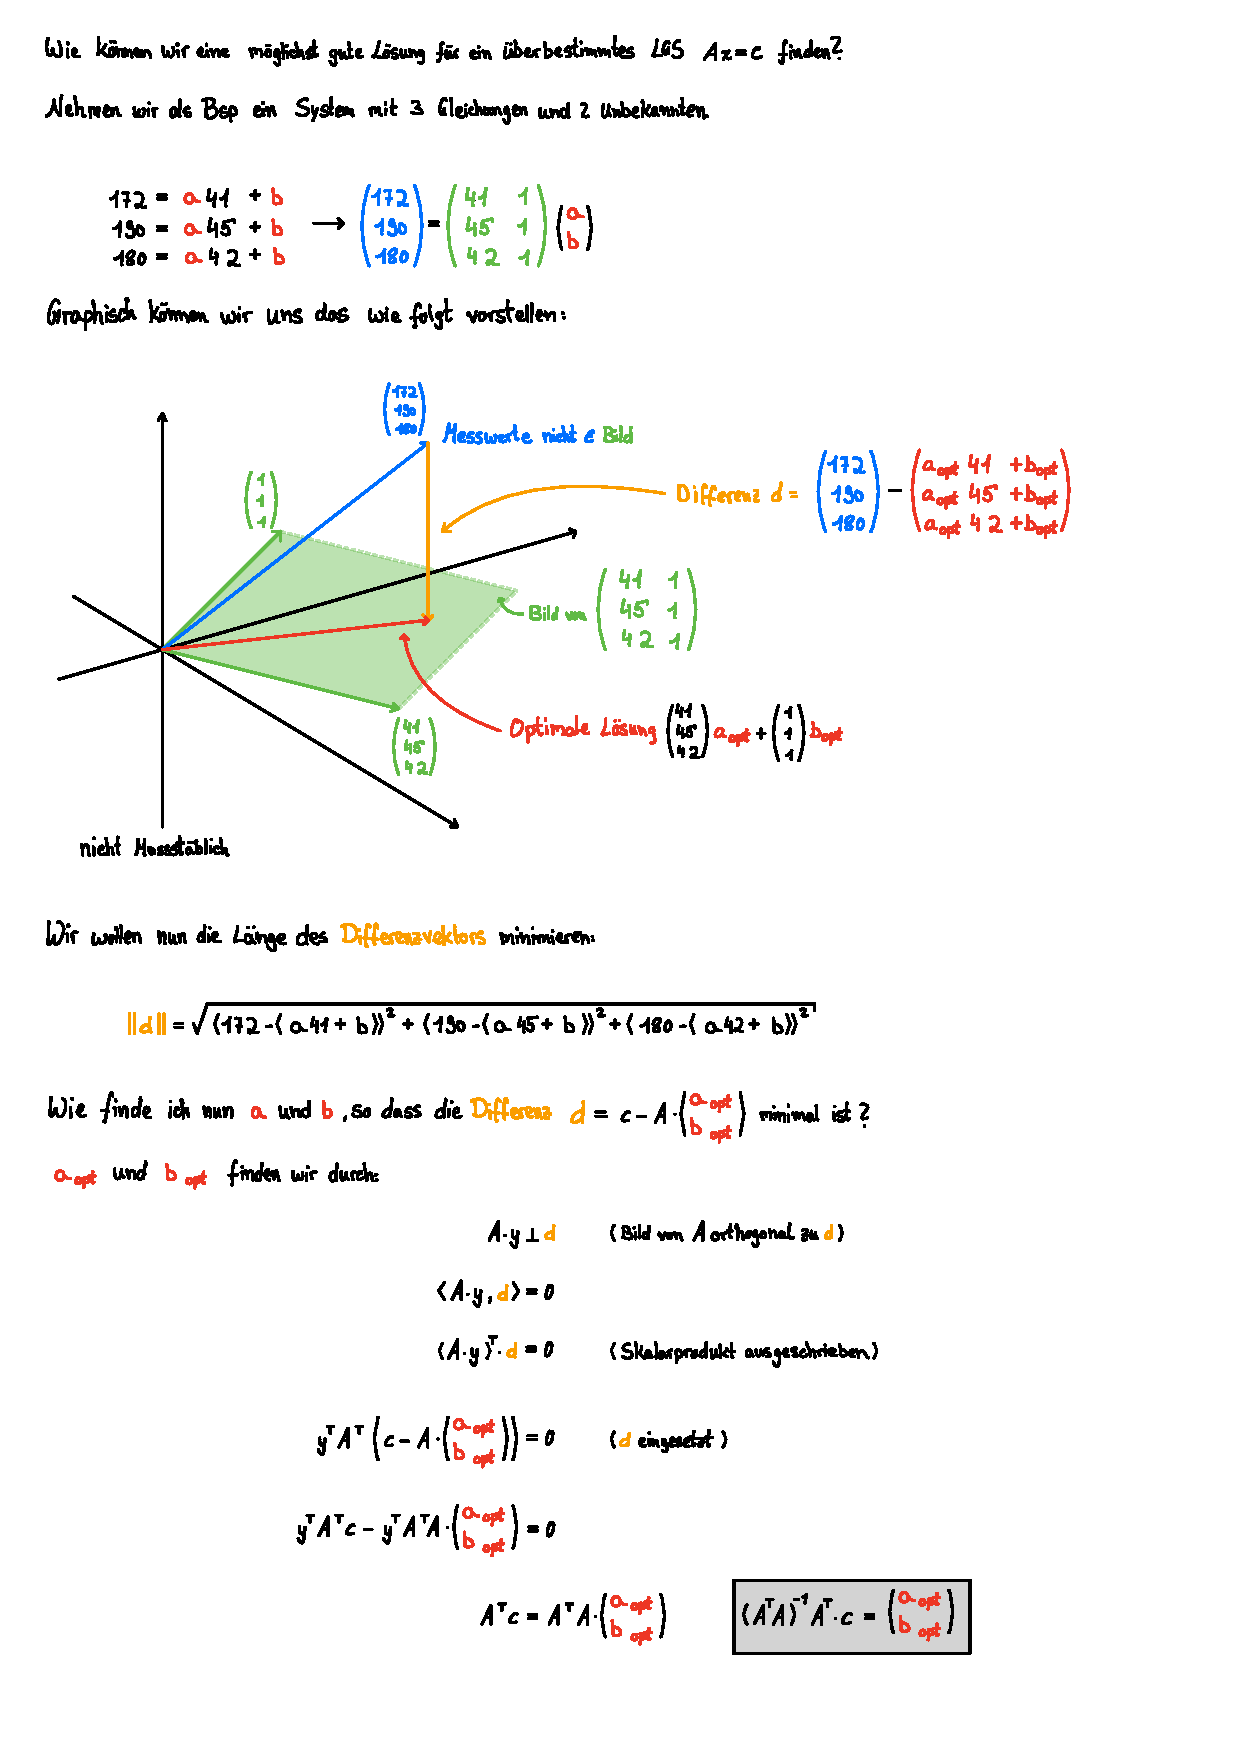
\includegraphics[page=1, scale=0.842]{pdf/07_Methode_der_kleinsten_Quarate.pdf}
\end{figure}
\newpage
\includepdf[pages={2-}, 
            pagecommand={\thispagestyle{plain}}, 
            scale=0.95]{pdf/07_Methode_der_kleinsten_Quarate.pdf}

\newgeometry{top=2.5cm, bottom=2cm}
\subsection{Beispielaufgaben} 
\vspace{1cm}
\subsubsection{} %Übung 09
Sei 
\[\begin{aligned}
 &x_1 +& 0&x_2 =& 2\\
 &x_1 +&  &x_2 =& 1\\
 &x_1 +& 2&x_2 =& 0\\
 &x_1 +& 3&x_2 =& -1\\
 &x_1 +& 4&x_2 =& 1\\
\end{aligned}\] \\
ein überbestimmtes lineares Gleichungssystem. Lösen Sie das Ausgleichproblem mittels der Methode der kleinsten Quadrate. Das heisst, finden Sie $(x_1,x_2)^\top$, so dass $\|r\|_2 = \|Ax-c\|_2$ minimal ist.\\

\noindent \textbf{Lösung:}

\newpage
\subsubsection{}
Gegeben sei
\[\begin{aligned}
 &x_1 +&  &x_2 &- 1 =&\; r_1\\
 &     &  &x_2 &- 3 =&\; r_2\\
 &     &  &x_2 &- 4 =&\; r_3\\
\end{aligned}\] \\
Lösen Sie das Ausgleichsproblem mittels der QR-Zerlegung. \\

\noindent \textbf{Lösung:}